
\documentclass[12pt,a4paper]{scrartcl}

\usepackage[a4paper, left=2cm, right=1cm, bottom=1cm, top=1cm, includeheadfoot]{geometry}
\usepackage[ngerman]{babel}
\usepackage[utf8]{inputenc} % comment this if you uncomment utf8x
%\usepackage[utf8x]{inputenc} % uncomment this if there are problems with 'ä', 'ü', 'ö'
\usepackage{ucs}
\usepackage[usenames,dvipsnames]{xcolor}
\usepackage[fleqn]{amsmath}
\usepackage{amsfonts}
\usepackage{amssymb}
\usepackage{color}
\usepackage{listings}
\usepackage{hyperref}
\usepackage{amsfonts}
\usepackage{listings}
\usepackage{scrpage2}
\usepackage{graphicx}


\definecolor{mygray}{rgb}{0.9,0.9,0.9}
\lstset{language=[Visual]Basic, morekeywords={param, local}}


\lstset{
   literate={ö}{{\"o}}1
           {ä}{{\"a}}1
           {ü}{{\"u}}1
           {ß}{{\ss}}1
           {é}{{\'e}}1,
   inputencoding=ansinew,
   extendedchars=true,
   basicstyle=\scriptsize\ttfamily,
   numberstyle=\scriptsize,
   breaklines=true,
   tabsize=2,
   numbersep=5pt
}
\lstdefinestyle{customcpp}{
   language=C++,
   backgroundcolor=\color{mygray},
   numbers=left,
   keywordstyle=\color{blue}\bfseries,
   stringstyle=\color{BrickRed}\ttfamily,
   commentstyle=\color{OliveGreen}\ttfamily,
   showspaces=false,
   showstringspaces=false,
   showtabs=false
}
\lstdefinestyle{customoutput}{
   backgroundcolor=\color{mygray},
   numbers=none,
   showspaces=false,
   showtabs=false
}

\newcommand{\sourceCode}[1]{\lstinputlisting[style=customcpp]{#1}} %beinhaltet alle benötigten Packages etc.
\begin{document}
\graphicspath{{./}}

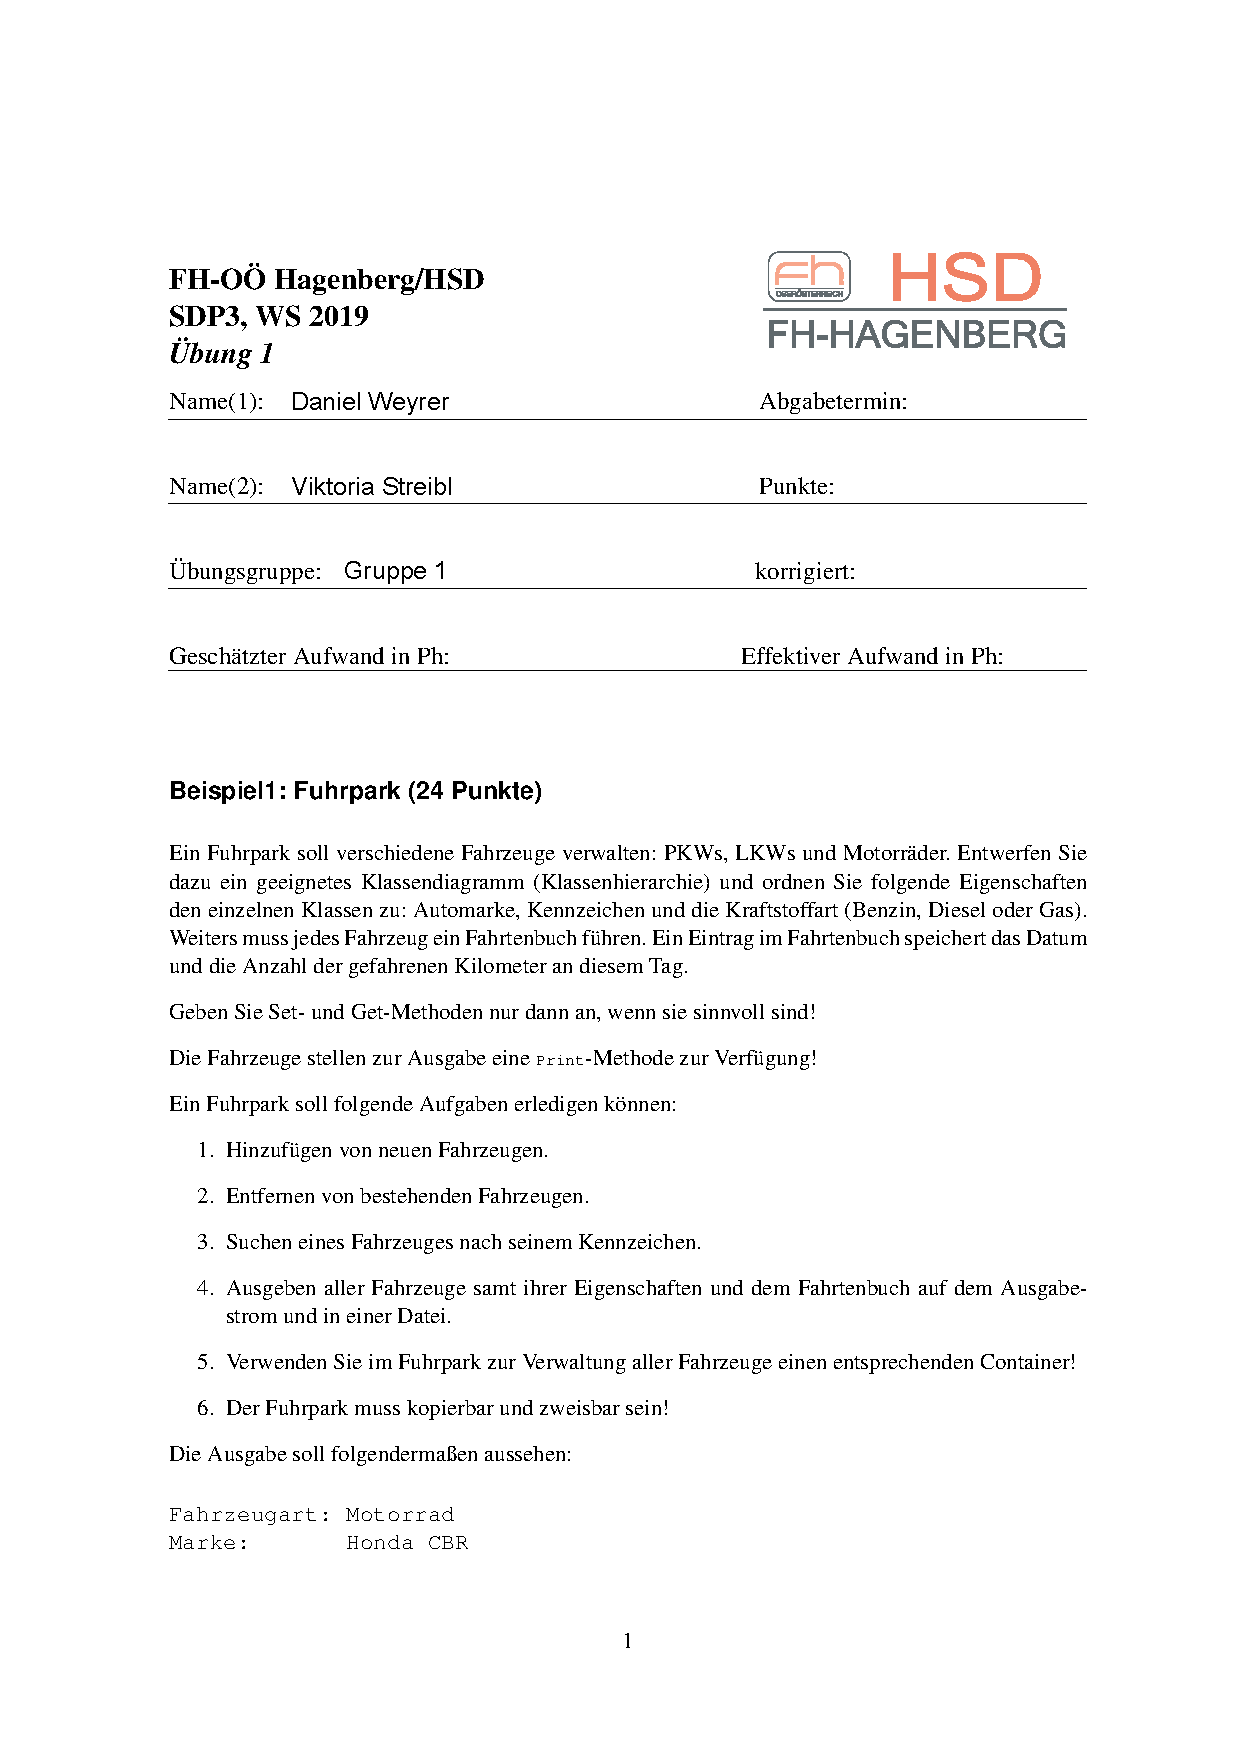
\includepdf[pages=-]{Angabe.pdf}

\title{SDP - Exercise 02} % Übungsname und Nummer angeben
\subtitle{winter semester 2019/20} % Semester angeben oder auskommentieren, falls nicht erwünscht
\author{
Viktoria Streibl - S1810306013\\
  Daniel Weyrer - S1820306044
} % Autorenname
\date{\today} % Das heutige Datum automatisch einfügen

\maketitle % Titelseite erstellen

\newpage
\tableofcontents % Inhaltsverzeichnis erstellen
\newpage

\ihead{Viktoria Streibl}
\ohead{Daniel Weyrer}
\chead{SDP3-UE Uebung 02}

\section{Organizational}
\subsection{Team}
\begin{itemize}
	\item Viktoria 	Streibl 		- 	S1810306013
	\item Daniel 	Weyrer		-	S1820306044
\end{itemize}

\subsection{Roles and responsibilities}

\subsubsection{Jointly}
\begin{itemize}
	\item planning
	\item Documentation
	\item Systemdocumentation
	\item Class Diagram
\end{itemize}

\subsubsection{Viktoria Streibl}
\begin{itemize}
	\item Main Class Company
	\item Interface ICompany
	\item Testdriver Client
	\item Main Testdriver
	
\end{itemize}

\subsubsection{Daniel Weyrer}
\begin{itemize}
	\item Base Class for Employee
	\item Derived Classes
		\subitem Class Commission Worker
		\subitem Class Hourly Worker
		\subitem Class Pieces Worker
		\subitem Class Boss
\end{itemize}

\subsection{Effort}

\subsubsection {Viktoria Streibl}
\begin{itemize}
	\item estimated: 10ph 
	\item actually: - ph
\end{itemize}

\subsubsection {Daniel Weyrer}
\begin{itemize}
	\item estimated: 10 ph 
	\item actually: - ph
\end{itemize}

\section{Requirenment Definition(System Specification)}
It was a company desired the various types of employees includes, such as commission worker, hourly worker, pieces worker and boss. Each employee type should also include and output some key data such as name, SSN, date of joining, salary and birthday. In addition, each company has to ouput the name and location.
Any number of employees can be added and deleted in the programm, but the client is not allowed to do so. It is possible to search for employees by nickname as well as by the type. The Client can also get all produces and all sold pieces.

\section{System Design}
\subsection{Classdiagram}
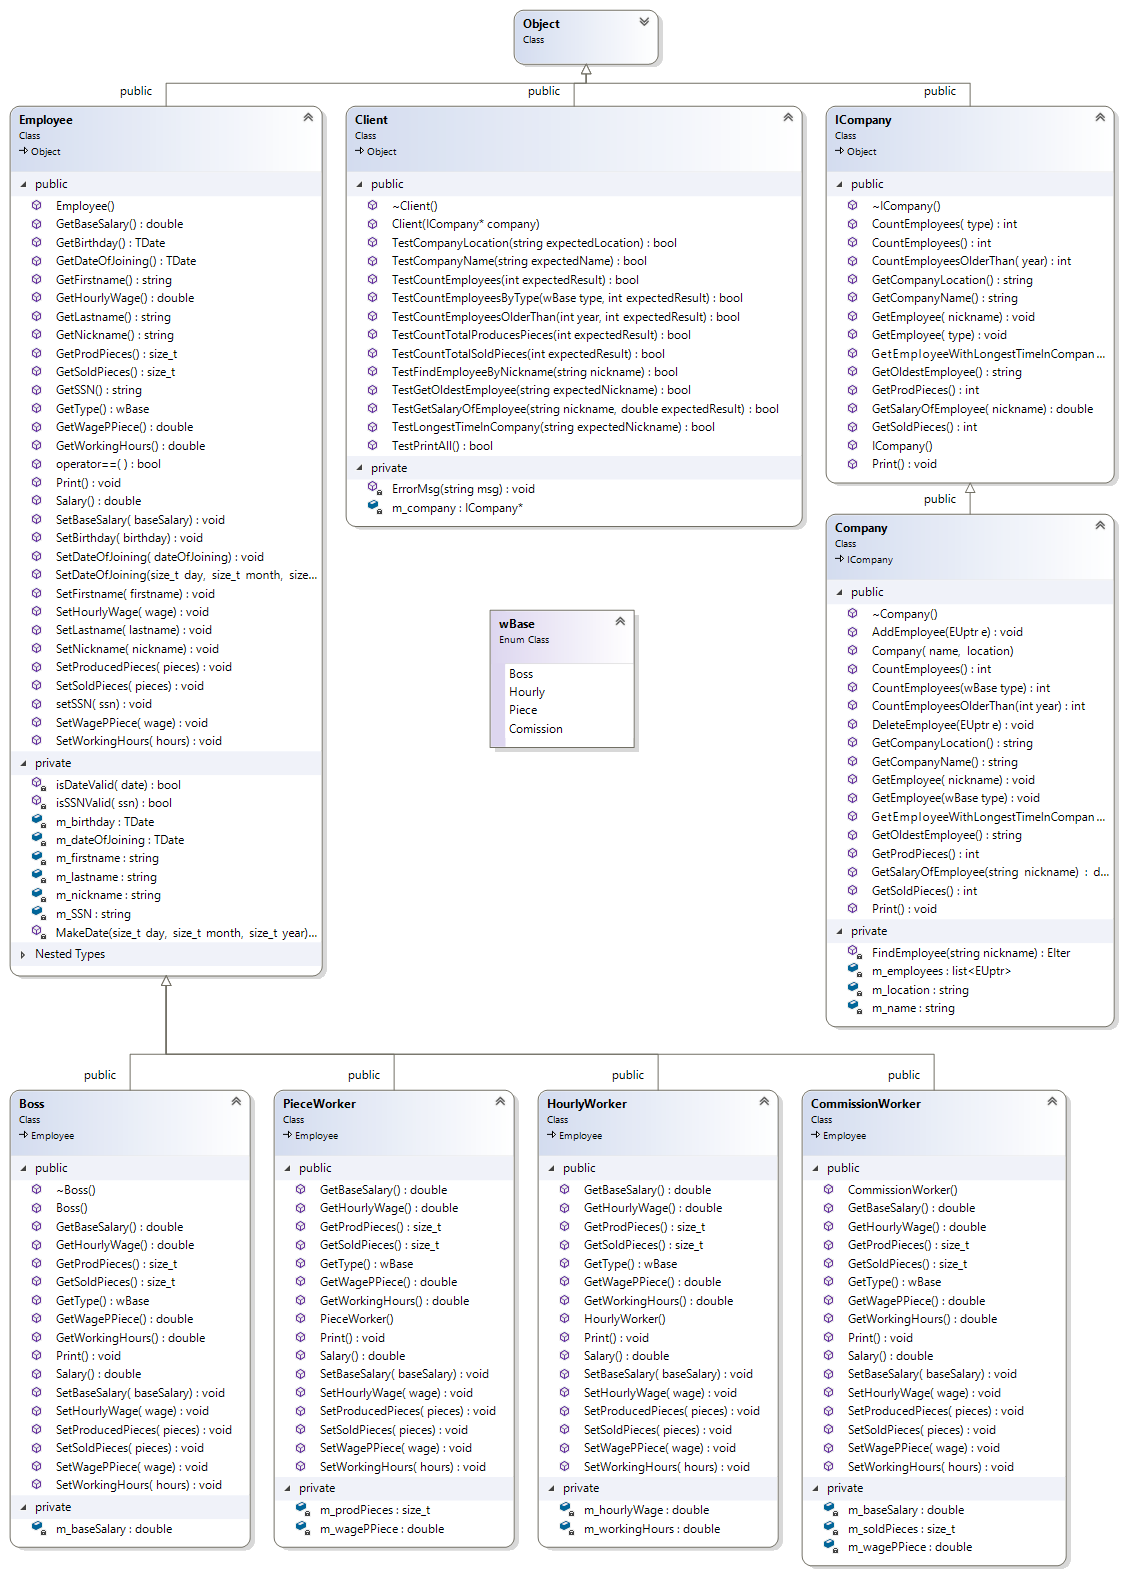
\includegraphics[scale=0.65]{ClassDiagram}

\subsection{Design Decisions}
\subsubsection{}
\subsubsection{}
\subsubsection{Search Employee}
Employee is searched by nickname because it has to be unique. To be sure that the nickname is unique we check it while adding new employee.

\section{Component Design}
\subsection{Class Client}
The Client simulate a person which use the interface.
The following functions tests the functionality:
\begin{itemize}
	\item Test the company name
	\item Test the company location
	\item Test if it is possible ot find a employee by nickname
	\item Test if it is possible ot find a employee by birthday
\end{itemize}

\subsection{Class ICompany}
Is an interface which is used by the Client.
It contains the following functions:
\begin{itemize}
	\item Get the company name
	\item Get the company location
	\item Get an employee by nickname
	\item Get employees by birthday
	\item Get all sold pieces
	\item Get all produced pieces
	\item Count all employees in the company
	\item Count all employees with the same age
	\item Ouput all employees in the company and some general data
\end{itemize}

The ICompany is the interface between an client and the company. The Client is not allowed to manipulate the employees.
It defines the methodes with can be used by the client.

"GetCompanyName", returns the name of the company.
"GetCompanyLocation", returns the location of the company.
"GetEmployee", can be used with the nickname or with the birthday and returns the employees.
"GetSoldPieces", counts all pieces which are sold by the company.
"GetProdPieces", counts all pieces which are produces by the employees.
"CountEmployees", returns the number of employees in the company.
"Print", outputs the name and location of the company, as well as all employees.

\subsection{Class Company}
Manages all employees in the company. It implements the interface ICompany.
It contains the following functions:
\begin{itemize}
	\item Add a new Employee
	\item Remove a Employee
	\item All functions from ICompany
\end{itemize}

The Company class manages all Employees. It uses unique pointers stored in a vector, to avoid shallow-copies.
With the method "AddEmploye" a new employee can be created. Should a employee already exist with the same nickname. So this employee is not stored and an error message output.
"DeleteEmployee" deletes a employee. If none is stored with the nickname an exception get`s thrown and caught in the same method.

\subsection{Class Employee}
Is the base class of all employee types.
It contains the following functions:
\begin{itemize}
	\item 
\end{itemize}

\subsection{Class CommissionWorker}
This class represents a comission worker.
\begin{itemize}
	\item
\end{itemize}

\subsection{Class HourlyWorker}
This class represents a hourly worker.
\begin{itemize}
	\item
\end{itemize}

\subsection{Class PiecesWorker}
This class represents a pieces worker.
\begin{itemize}
	\item
\end{itemize}

\subsection{Class Boss}
This class represents a boss.
\begin{itemize}
	\item
\end{itemize}

\subsection{TestDriver}
The Testdriver test alle functions of the Client. It adds commisson worker, hourly worker, pieces worker and a boss and deletes them.
It searches employees by nickname and birthday and print all of them.

\newpage
\section{Test Protocol}
It has been tested in the file "TestDriver", the following points have been tested:
\begin{itemize}
	\item 
\end{itemize}

\subsection{Console Output}
\sourceCode{./CalcSalary/output.txt}
\newpage

\section{Source Code}


\subsection{Class Client}
\subsubsection{Client.h}
\sourceCode{./CalcSalary/CalcSalary/Client.h}
\newpage
\subsubsection{Client.cpp}
\sourceCode{./CalcSalary/CalcSalary/Client.cpp}

\subsection{Interface ICompany}
\subsubsection{ICompany.h}
\sourceCode{./CalcSalary/CalcSalary/ICompany.h}

\subsection{Class Company}
\subsubsection{Company.h}
\sourceCode{./CalcSalary/CalcSalary/Company.h}
\subsubsection{Company.cpp}
\sourceCode{./CalcSalary/CalcSalary/Company.cpp}

\subsection{Class Employee}
\subsubsection{Employee.h}
\sourceCode{./CalcSalary/CalcSalary/Employee.h}
\subsubsection{Employee.cpp}
\sourceCode{./CalcSalary/CalcSalary/Employee.cpp}

\newpage
\subsection{Class CommissionWorker}
\subsubsection{CommissionWorker.h}
\sourceCode{./CalcSalary/CalcSalary/CommissionWorker.h}
\newpage
\subsubsection{CommissionWorker.cpp}
\sourceCode{./CalcSalary/CalcSalary/CommissionWorker.cpp}

\subsection{Class HourlyWorker}
\subsubsection{HourlyWorker.h}
\sourceCode{./CalcSalary/CalcSalary/HourlyWorker.h}
\newpage
\subsubsection{HourlyWorker.cpp}
\sourceCode{./CalcSalary/CalcSalary/HourlyWorker.cpp}

\subsection{Class PieceWorker}
\subsubsection{PieceWorker.h}
\sourceCode{./CalcSalary/CalcSalary/PieceWorker.h}
\newpage
\subsubsection{PieceWorker.cpp}
\sourceCode{./CalcSalary/CalcSalary/PieceWorker.cpp}

\subsection{Class Boss}
\subsubsection{Boss.h}
\sourceCode{./CalcSalary/CalcSalary/Boss.h}
\newpage
\subsubsection{Boss.cpp}
\sourceCode{./CalcSalary/CalcSalary/Boss.cpp}

\subsubsection{TestDriver.cpp}
\sourceCode{./CalcSalary/CalcSalary/TestDriver.cpp}

% Um Quellcode einzufügen einfach diesen Befehl verwenden:
%\sourceCode{Relativer/Pfad/zum/SourceCode.Endung}

\end{document}